The goal is to transform the ``problematic'' term in \eref{recurrence}, \ie, the power term defined by \eref{power-model}, in such a way that the recurrence in \eref{recurrence} becomes computationally tractable.
Our solution is the construction of a surrogate model for the power model in \eref{power-model}, which we further propagate through \eref{recurrence} to obtain an approximation for temperature.
To this end, we employ polynomial chaos (PC) expansions \cite{xiu2010}, which decompose stochastic quantities into infinite series of orthogonal polynomials of random variables.
Such series are especially attractive from the post-processing perspective as they are nothing more than polynomials; hence, PC expansions are easy to interpret and evaluate.
An introduction to orthogonal polynomials is given in the appendix, \aref{orthogonal-polynomials}.

\begin{figure}
  \centering
  \updatedFigure{
  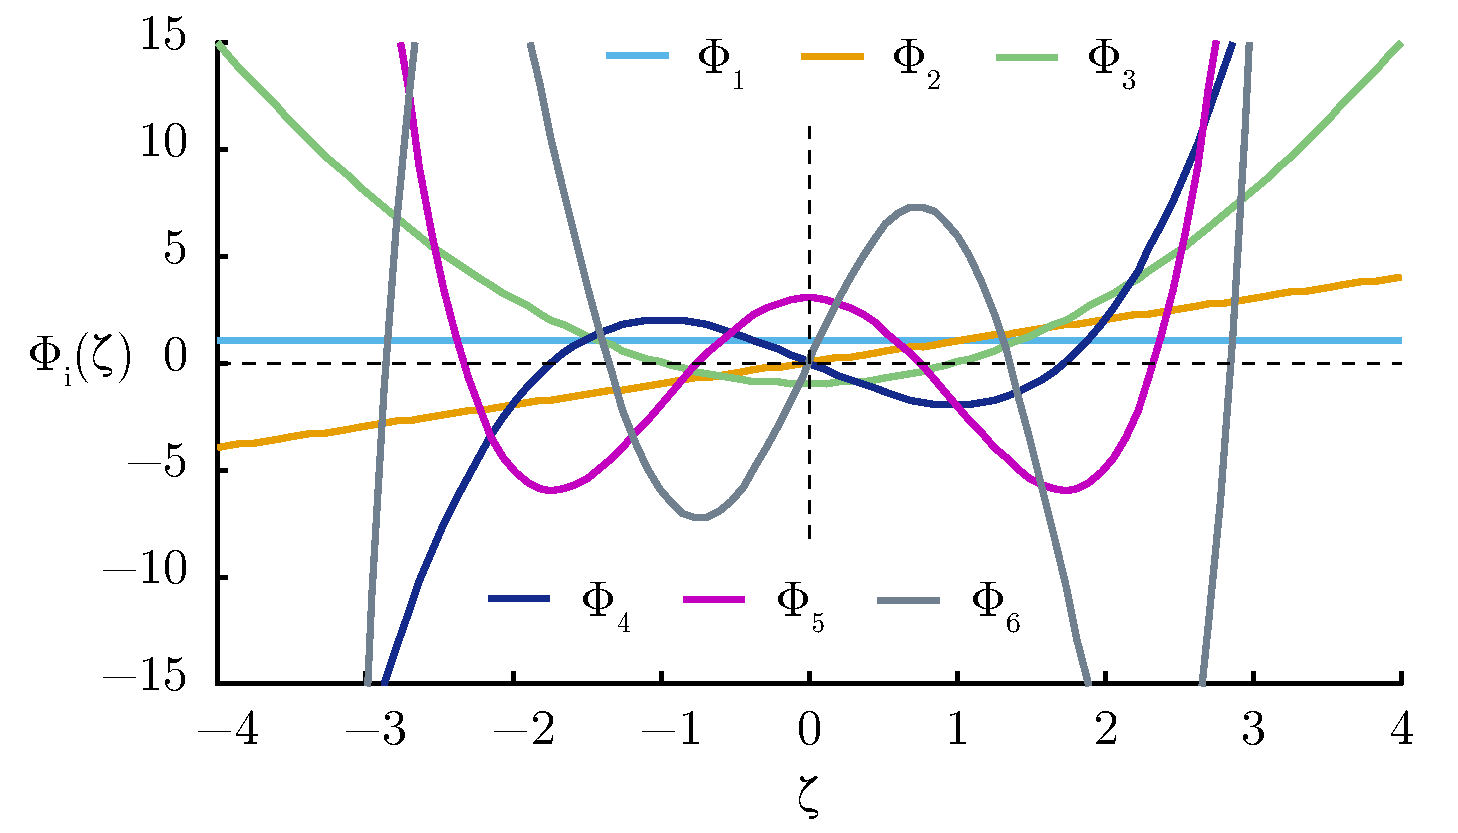
\includegraphics[width=0.9\columnwidth]{include/assets/hermite.pdf}
  }
  \vspace{-1.0em}
  \caption{The first six polynomials of the Hermite basis.}
  \vspace{-1.5em}
  \flabel{hermite}
\end{figure}

The first step towards a PC expansion is the choice of a suitable polynomial basis $\{ \pcb_i(\vz) \}_{i = 1}^\infty$, which is typically picked from the Askey scheme of orthogonal polynomials \cite{xiu2010}.
The step is crucial as the rate of convergence of PC expansions closely depends on it.
Although there are no strict rules that guarantee the optimal choice \cite{maitre2010, knio2006}, there are best practices which say that one should be guided by the probability distributions of the (independent) random variables that drive the stochastic system at hand (see \aref{polynomial-chaos}).
In our case, these variables are $\vZ(\o)$.
\tref{askey} in the appendix displays several examples of such paired probability distributions and polynomial bases.
For instance, when a random variable follows a beta distribution, the Jacobi basis is worth being tried first; on the other hand, the Hermite basis is preferable for Gaussian distributions.
In order to give a better intuition of what such a basis may look like, \fref{hermite} shows the first six polynomials $\{ \pcb_i(\z) \}_{i = 1}^6$, $\z \in \real$, of the Hermite basis in the one-dimensional scenario.
Since $\vZ(\o)$ is an $\nvars$-dimensional random variables, several (possibly different) one-variate bases are to be combined together to produce a single $\nvars$-variate polynomial basis $\{ \pcb_i(\vz) \}_{i = 1}^\infty$, $\vz \in \real^\nvars$ (see \cite{xiu2010, maitre2010}).

Having an appropriate basis chosen, we apply the PC procedure to power in \eref{recurrence} and truncate the resulting infinite series in order to make it feasible for practical implementations. Such an expansion is formally defined as
\begin{equation} \elabel{pc-expansion}
  \oPC{\nvars}{\pcorder}{\vP_k(\o)} := \sum_{i = 1}^{\pcterms} \pcc{\vP}_{ki} \; \pcb_i(\vZ(\o))
\end{equation}
where $\{ \pcb_i(\vz) \}_{i = 1}^{\pcterms}$, $\vz \in \real^\nvars$, is the truncated basis with $\pcterms$ polynomial terms of $\nvars$ variables, and $\pcc{\vP}_{ki} \in \real^\nprocs$ are the coefficients of the expansion. The latter are computed using spectral projections as it is explained in the appendix, \aref{spectral-projection}.
$\pcorder$ denotes the order of the expansion, which determines the maximal degree of the $\nvars$-variate polynomials involved in the expansion, which directly translates into $\pcterms$; hence, $\pcorder$ also determines the resulting accuracy of the expansion.

It can be seen in \eref{recurrence} that, due to the linearity of the operations involved in the recurrence, $\vX_k(\o)$ retains the same polynomial structure as $\vP_k(\o)$. Therefore, using \eref{pc-expansion}, \eref{recurrence} is rewritten as follows, for $k = 1, \dotsc, \nsteps$:
\begin{equation} \elabel{expanded-recurrence}
  \oPC{\nvars}{\pcorder}{\vX_k(\o)} = \mCF_k \: \oPC{\nvars}{\pcorder}{\vX_{k-1}(\o)} + \mCS_k \: \oPC{\nvars}{\pcorder}{\vP_k(\o)}.
\end{equation}
Thus, there are two PC expansions for two concurrent stochastic processes with the same basis but different coefficients. As shown in \aref{spectral-projection}, \eref{expanded-recurrence} can be reduced to
\begin{equation} \elabel{pc-recurrence}
  \pcc{\vX}_{ki} = \mCF_k \: \pcc{\vX}_{(k - 1)i} + \mCS_k \: \pcc{\vP}_{ki}
\end{equation}
where $k = 1, \dotsc, \nsteps$ and $i = 1, \dotsc, \pcterms$. Finally, \eref{fourier-output} and \eref{pc-recurrence} are combined together to compute the coefficients of the PC expansion of the temperature vector $\vTO_k(\o)$.

To summarize, let us recall the stochastic recurrence in \eref{recurrence} where, in the presence of correlations, an arbitrary functional $\vP_k(\omega)$ of the uncertain parameters $\vU(\o)$ and random temperature $\vTO_k(\o)$ (see \sref{power-model}) needs to be evaluated and combined with another random vector, $\vX_k(\omega)$.
Now, the recurrence in \eref{recurrence} has been replaced with a purely deterministic recurrence in \eref{pc-recurrence} that involves only linear operations.
Moreover, the performed spectral decompositions have substituted the heavy thermal system in \eref{fourier-system} with a light polynomial surrogate defined by a set of basis functions $\{ \pcb_i(\vz) \}_{i = 1}^\pcterms$ and the corresponding sets of coefficients, namely, $\{ \pcc{\vP}_{ki} \}_{i = 1}^\pcterms$ for power and $\{ \pcc{\vTO}_{ki} \}_{i = 1}^\pcterms$ for temperature, where $k$ traverses all the $\nsteps$ intervals of the considered time span.
Consequently, the output of the proposed framework constitutes two stochastic profiles: the power and temperature profiles denoted by $\profileP{\o}$ and $\profileT{\o}$, respectively, which are ready to be analyzed.
